\documentclass[12pt, a4paper, onecolumn]{IEEEtran}
% https://www.monash.edu/rlo/quick-study-guides/writing-a-case-study
\usepackage{url} % for typesetting URLs
\usepackage{hyperref}
\usepackage{cleveref}
\hypersetup{
	colorlinks=true,
	linkcolor=blue,
	filecolor=blue,
	citecolor=blue,
	urlcolor=magenta,
}
\usepackage[style=ieee]{biblatex}

% Citation Needed Command
\usepackage{xcolor}
\newcommand{\citationneeded}{[\textcolor{blue}{citation needed}]}

\usepackage{caption}
\usepackage{subcaption}
\usepackage{graphicx}
\graphicspath{ {./pictures/} }

%% Bibliography
\addbibresource{./bibliography.bib}

\title{An Overview of Chordophone Actuation}
\author{Joshua Benfell}

\begin{document}

	\maketitle
    \section{Introduction}
        Humans are mechanically fluid and complex with the ability to produce a wide range of minute differences of similar motions. 
        As such, many methods of picking a stringed instrument are present, from the picking of individual strings to strumming. 
        Similar methods further vary in expressiveness due to properties such as the angle of attack and volume.
        Such a wide range of possibilities is reflected in the variation of existing mechanisms.
        Furthermore, damping strings, to prevent certain tones, is an integral part of playing instruments due to the dynamics introduced.
    \section{Picking Mechanisms}

        \begin{figure}[!h]
            \centering
            \begin{subfigure}{0.3\textwidth}
                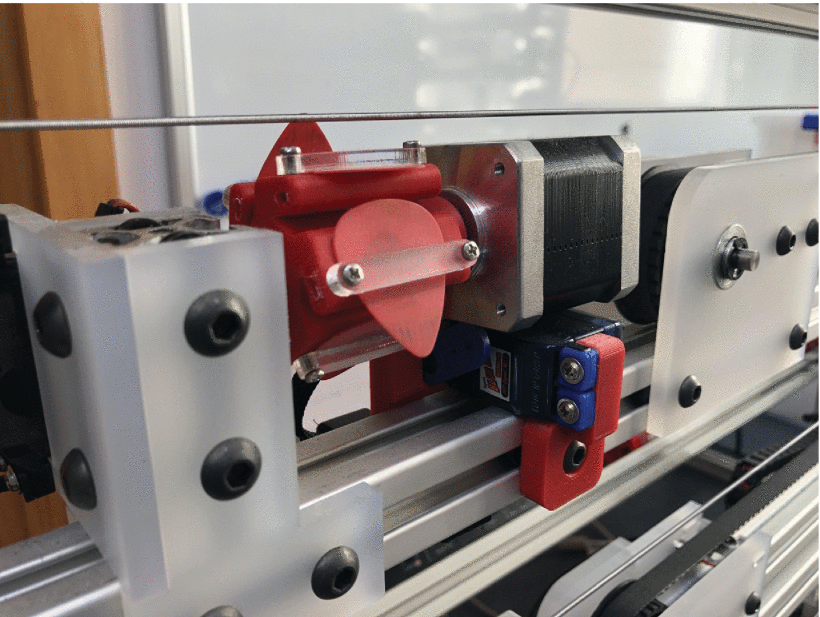
\includegraphics[width=\columnwidth]{mechbass_picking.png}
                \subcaption{Mechbass Picking Mechanism \cite{VUW_Chordophones}}
                \label{fig:mechbass_picking}
            \end{subfigure}
            \begin{subfigure}{0.2\textwidth}
                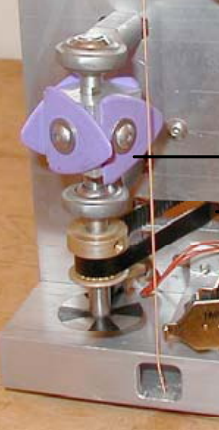
\includegraphics[width=\columnwidth]{guitarbot_picking.png}
                \subcaption{GuitarBot Picking Mechanism \cite{GuitarBot}}
                \label{fig:guitarbot_picking}
            \end{subfigure}
            \caption{Rotary Picking Mechanisms}
            \label{fig:RotaryPicking}
        \end{figure}

        
        Mechanisms for picking individual strings most commonly consist of a drum that rotates multiple plectra, as seen with Mechbass \cite{VUW_Chordophones}, GuitarBot \cite{GuitarBot} and Tempo Mecho \cite{barton_2019}, or the use of a solenoid to actuate a plectra over a string \cite{PWM_Solenoid,Silent_Picking,Pivot_Picking}. 
        Rotary mechanisms (\Cref{fig:RotaryPicking}) make use of a drum of equally spaced plectra that rotates to strike the string.
        Solenoid based picking methods, work by using one (\Cref{fig:silent_picking}) or two (\Cref{fig:pwm_picking}) solenoids to push and pull a plectra over a string.
        As is evident in \Cref{fig:SolenoidPicking}, these are generally considerably larger than the rotary variant.
        
        \begin{figure}[!h]
            \centering
            \begin{subfigure}{0.2\textwidth}
                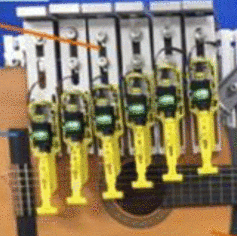
\includegraphics[width=\columnwidth]{silent_picking.png}
                \subcaption{\cite{Silent_Picking}}
                \label{fig:silent_picking}
            \end{subfigure}
            \begin{subfigure}{0.3\textwidth}
                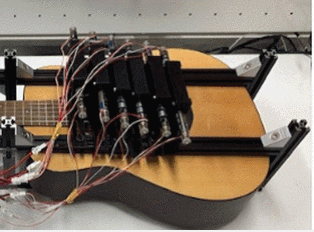
\includegraphics[width=\columnwidth]{pwmSolenoid_picking.png}
                \subcaption{\cite{PWM_Solenoid}}
                \label{fig:pwm_picking}
            \end{subfigure}
            \begin{subfigure}{0.3\textwidth}
                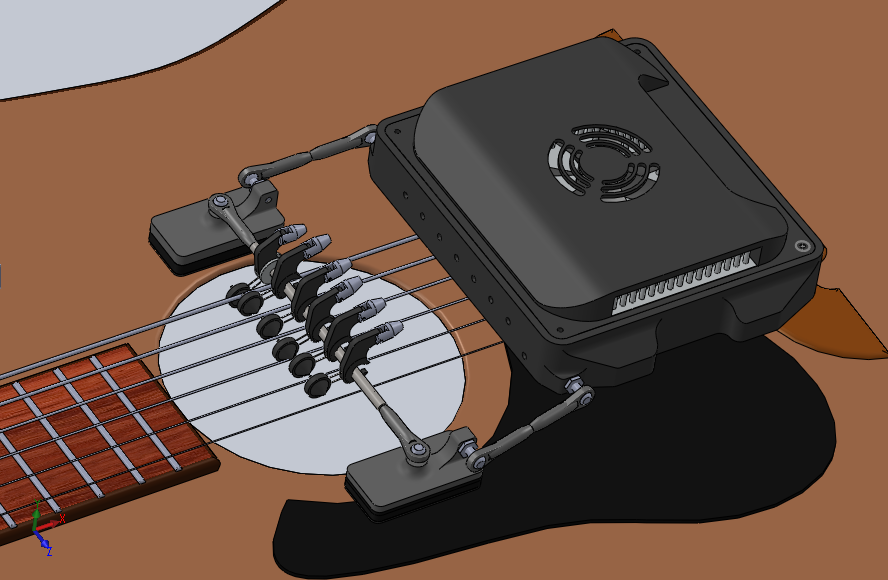
\includegraphics[width=\columnwidth]{pivotSolenoid_picking.png}
                \subcaption{\cite{Pivot_Picking}}
                \label{fig:pivot_picking}
            \end{subfigure}
            \caption{Solenoid Based Picking Mechanisms}
            \label{fig:SolenoidPicking}
        \end{figure}

        Both of these types of picking mechanism are both capable of speeds greater than what is reasonably acheivable from humans \cite{pickspeed}. 
        Rotary methods have greater design flexibility as increasing the drum size increases the maximum picking speed through an increase in pick count and speed \cite{VUW_Chordophones,pickspeed}.
        In contrast, solenoids have fixed speeds per model, making an increase require a different actuator, with slower speeds capable through the use of PWM control \cite{PWM_Solenoid}.
        However, rotary methods require aligning multiple plectra so that the sound is consistent through a full rotation.

        When it comes to physical size, the solenoid mechanisms take up considerably more space than the rotary counterpart as they are typically designed across the string \cite{VUW_Chordophones,Silent_Picking,PWM_Solenoid}.
        However, by changing the pick and the picking direction, it is possible to reduce the size of the actuator \cite{Pivot_Picking}.
        As this design was capable of fitting on the guitar adjacently, it is possible, that a solenoid actuator could be suited to monochord setups.
        However, the ability to vary the way the pick strikes is sacrificed.

        Due to the ability to vary the speed at which the plectra crosses the string, the two groups of actuation are capable of varying the volume of the sound produced, with higher speeds resulting in higher volumes \cite{PWM_Solenoid}.
        However, what they lack is the ability to change how the pick crosses the string.
        Mechbass utilises a servo to move the picker, altering where the plectra strikes the string, with closer causing an increased volume \cite{VUW_Chordophones}. 
        Further expressiveness can be added by changing the attack angle. 
        % Neither of these adjustments have been attempted with solenoids, however, this is due to the rotary system being simpler to move and adjust due to the size and layout.

        Actuating strings introduces many noise sources, both electromagnetic and mechanial, which will effect the performance.
        Both motor types can be picked up by magnetic pickups, so it is important to place these well to reduce this without introducing weakness or altering the sound significantly, or use different transducers \cite{VUW_Chordophones}.
        Further, to reduce mechanical noise in solenoids, an elastic membrance can be used to reduce the impact of solenoids \cite{Silent_Picking}.

        
    \section{Damping Mechanisms}
        Damping mechanisms consist of a servo or solenoid with foam, felt or silicone making contact with the string, with silicone being the most like human skin \cite{VUW_Chordophones}.
        They have been used at points near the picking mechanism, and the pitch shifter, as these create different results \cite{VUW_Chordophones}.
        Typically these have been used to fully mute strings, however, it is possible to partially mute, with lighter touches.
        Where these mechanisms fall short is in controlled decay of the sound, as they have only been used to move to set positions.
        Further development for damping mechanisms would be to explore playing actively with the damping through slap muting.


    \section{Conclusion}
        NOne that does all the actuation
        EM noise
        Study into Stepper noise
        Slap muting
        Rotary attached to chorded guitar

    \printbibliography

\end{document}